\documentclass[problem]{mcs}

\begin{pcomments}
\pcomment{FP_uniform_stationary_distribution}
\pcomment{from: S08.final}
\end{pcomments}

\pkeywords{
  random_walk
  uniform
  stationary_distribution  
}

%%%%%%%%%%%%%%%%%%%%%%%%%%%%%%%%%%%%%%%%%%%%%%%%%%%%%%%%%%%%%%%%%%%%%
% Problem starts here
%%%%%%%%%%%%%%%%%%%%%%%%%%%%%%%%%%%%%%%%%%%%%%%%%%%%%%%%%%%%%%%%%%%%%

\begin{problem}
  For which of the following graphs is the uniform distribution over
  nodes a stationary distribution?  The edges are labeled with
  transition probabilities.  Explain your reasoning.

\begin{figure}
\subfloat{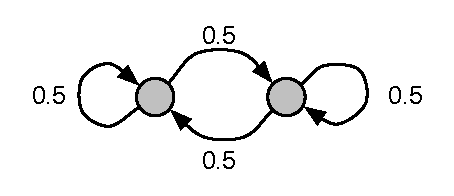
\includegraphics[height=1in]{sttnry0}}
\qquad
\subfloat{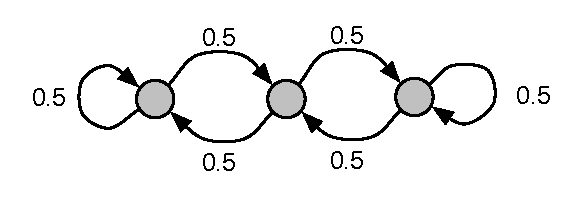
\includegraphics[height=1in]{sttnry1}}

\subfloat{
\includegraphics[height=1in]{sttnry2}}
\qquad
\subfloat{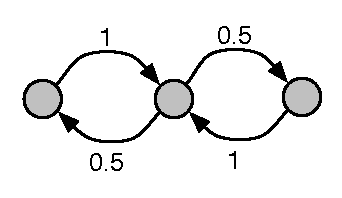
\includegraphics[height=1in]{sttnry3}}
\end{figure}

\begin{solution}
    All except the last one (bottom right). 

    One way of approaching this problem is by performing a single
    update step according to the rule
    \[ \widehat{d}(v) = \sum_{u\;\text{s.t.}\;\diredge{u}{v}} d(u)
    p(u,v), \]
    where $d$ is the stationary distribution ($1/2$ for all vertices
    on the left graphs, $1/3$ for all vertices on the right),
    $\widehat{d}$ is the distribution after one step, and $p(u,v)$ is the
    edge probability.  If $\widehat{d} = d$, then by definition, the
    uniform distribution is stationary.

    Alternatively, you could observe that the uniform distribution is
    stationary if and only if $\widehat{d}(v) = d(v)$, and hence dividing
    both sides by probability of being at each vertex, we get 
    \[ 1 = \sum_{u\;\text{s.t.}\;\diredge{u}{v}} p(u,v). \]
    In other words, the uniform distribution is stationary if and only
    if the incoming-edge probabilities sum to 1.
\end{solution}

\end{problem}

\endinput
